\todo[inline]{ausführtlicher da anscheinend doch nicht ganz unwichtig für die klausur}
Es wird in vielen Modellen eine Schichtenstruktur übernommen, wie sie bspw. in der Großhirnrinde zu finden ist.\\
Neuron besteht aus Zellkörper, Dendriten und Axon. Nervenimpuls breitet sich vom Axonhügel über gesamtes Axon aus.\\
Synapsen sind die Kopplungen zwischen Neuronen.\\
Das Ruhepotential liegt bei ca. $-75\si{\milli \volt}$. Spikes haben Amplitude bis ca. $+30\si{\milli \volt}$. Danach leichtes Unterschwingen bis Ruhepotential wieder erreicht wird.\\
Am Neuron werden die Aktionspotentiale zeitlich und räumliche summiert/integriert. Wenn Schwellwert erreicht wird, feuert das Neuron.

\section{Neuronale Verarbeitung}
\begin{enumerate}
    \item NN bestehen aus Neuronen, welche über Synapsen verbunden sind
    \item Neuronen senden über Axon Aktionspotentiale aus
    \item Neuronen summieren/integrieren ankommende AP auf
    \item wird Schwellwert überschritten feuert Neuron\\
        wird Schwellwert nicht überschritten feuert Neuron nicht
\end{enumerate}

\section{Hodgkin-Huxley Modell}
\begin{itemize}
    \item es handelt sich hierbei um ein komplexes Neuronenmodell
    \item neurophysiologische Experimente an Zellmembran von Tintenfisch als Grundlage $\rightarrow$ Erkenntnisse zu Ruhepotential und Weiterleitung der AP
    \item Modell enthält Charakteristika der Ionen-Kanäle
\end{itemize}
$\rightarrow$ Auf Grund der hohen Komplexität nicht für große Netze geeignet


\subsection{Ersatzschaltbild der Axonmembran}
In \ref{ch_bio_esb} ist das ESB für die Axonmembran zu sehen. Es werden die Kalium-, Natrium-,Leck/Chloridströme modelliert. Die Membrankapazität wird durch einen Kondensator modelliert. Der Gesamtstrom ergibt sich als Summe der drei Teilströme 
\begin{equation*}
    I_{Ionen} = I_K + I_{Na} + I_L = G_K(U-E_K) + G_{Na}(U-E_{Na}) + G_L(U-E_L)
\end{equation*}
Das Membranpotential ist durch die DGL
\begin{equation*}
    C\frac{dU}{dt} = I_{ext}-I_{Ionen}
\end{equation*}
gegeben, wobei $I_{ext}$ ein externer Strom ist. Die oben verwendeten Größen selbst werden alle wieder erneut durch DGLn beschrieben.\\
$\rightarrow$ Es können keine analytischen Lösungen bestimmt werden.\\
Das Modell beschreibt das biologische Vorbild recht gut. (siehe Skript für genaue Ergebnisse)\\
In der Praxis ist das Modell zu komplex und rechenintensiv.


\begin{figure}[h]
    \centering
    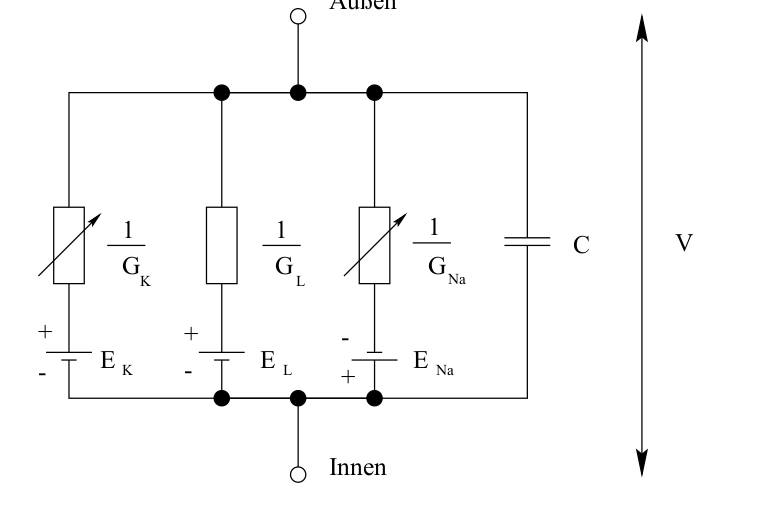
\includegraphics[width=0.75\textwidth]{img/BiologischesModell/ESB.png}
    \caption{Ersatzschaltbild für Axonmembran}
    \label{ch_bio_esb}
\end{figure}


\section{Kontinuierliches Modell}
\begin{itemize}
    \item keine Modellierung der einzelnen Ionen-Kanäle mehr
    \item Beschreibung eines Neurons durch zwei Gleichungen
        \begin{itemize}
            \item DGL dentritisches Membranpotential $u_j(t)$
            \item Axonales Membranpotential durch Funktionsauswertung $y_j(t)=f(u_j(t))$
        \end{itemize}
    \item synaptische Kopplungen werden durch reelle Zahlen $c_{ij}$ beschrieben.
    \item räumliche und zeitliche Integration: Summation der AP nach Gewichtung mit synaptischen Kopplungsstärken
\end{itemize}

\subsection{Modellgleichung}
\begin{align*}
    \tau \Dot{u}_j(t) & = -u_j(t) + x_j(t) + \sum_{i=1}^n c_{ij}y_i(t-d_{ij})\\
    y_j(t) &= f_j(u_j(t))
\end{align*}

Hierbei ist $\tau$ eine Zeitkonstante $>0$. $u_j(t)$ das dentritische Potential. $x_j(t)$ der externe Input. $c_{ij}$ die synaptische Kopplungsstärke. $d_{ij}$ die Laufzeit. $y_j(t)$ das axonale Potential und $f_j(x)$ die j-te Transferfunktion.\\

Auch diese DGL ist nicht analytische lösbar. Es kann aber eine Näherungslösung bestimmt werden durch diskretisieren der Zeit. Es ergibt sich dann

\begin{equation*}
    \Dot{u}_j(t) = \frac{u_j(t+\Delta t)-u_j(t)}{\Delta t}
\end{equation*}

daraus ergeben sich die 

\subsubsection{Diskrete Modellgleichungen}
\begin{align*}
    \frac{\tau}{\Delta t}(u_j(t+\Delta t)-u_j(t)) & = -u_j(t) + x_j(t) + \sum_{i=1}^n c_{ij}y_i(t-d_{ij})\\
    y_j(t) &= f(u_j(t))
\end{align*}

\subsection{Einfache Transferfunktionen}
\begin{itemize}
    \item Lin. Fkt $f(x) = x$ $\rightarrow$ lineares Neuron
    \item Heavisidefunktion $\rightarrow$ Schwellwertneuron
    \item Stückweise lineare Funktion $f (x) = \left\{
                                        \begin{array}{ll}
                                        0 & x \leq 0 \\
                                        x & \, x\in[0,1] \\
                                        1 & x\geq 1
                                        \end{array}
                                        \right. $
    \item logistische Funktion $f(x) = \frac{1}{1+\exp{-\beta x}}$                         
\end{itemize}

Die Funktionen (2)-(4) liegen im Wertebereich $[0,1]$. Es kann aber auch der Wertebereich $[-1,1]$ wünschenswert sein (dann bspw. mit Tanh).

\subsection{Neuronenmodell in Anwendungen}
\begin{figure}[h]
    \centering
    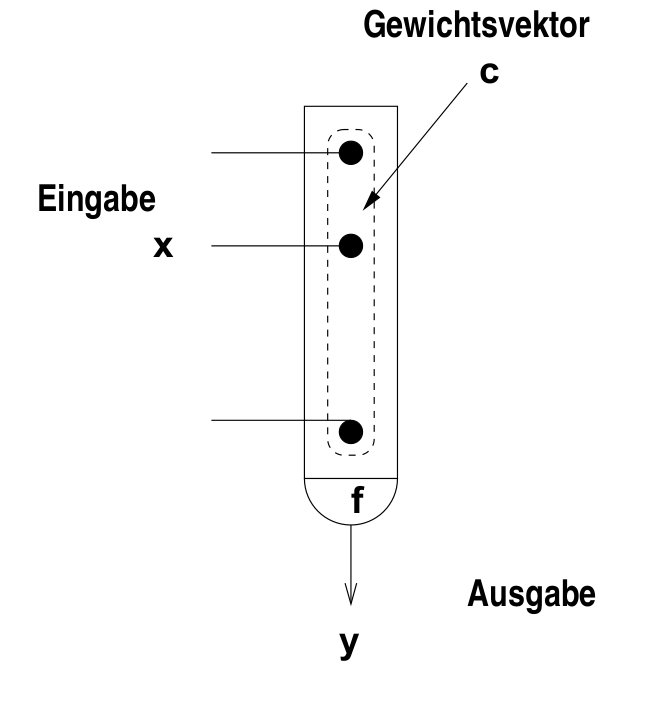
\includegraphics[width=0.25\textwidth]{img/BiologischesModell/NeuronenmodellAnwedung.png}
    \caption{Neuronenmodell in Anwedungen}
    \label{ch_bio_nmAnwendung}
\end{figure}

Für das Neuronenmodell in Anwendungen werden die folgenden Vereinfachungen gemacht
\begin{itemize}
    \item Neuronen ohne Gedächnis
    \item vernachlässigen der Signallaufzeit $d_{ij}$
\end{itemize}
Einige Beispiele

\paragraph{Lineares Neuron}
\begin{equation*}
    y(x) = \langle x,c \rangle + \Theta = \sum_{i=0}^n x_ic_i + \Theta
\end{equation*}

\paragraph{Schwellwert Neuron}
\begin{equation*}
    y (x) = \left\{
                                        \begin{array}{ll}
                                        1 & \,\langle x,c \rangle \geq \Theta \\
                                        0 & \, \text{sonst} \\
                                        \end{array}
                                        \right. 
\end{equation*}

\paragraph{Kontinuerliches nicht lineares Neuron}
\begin{equation*}
    y(x) = f(\langle x,c \rangle + \Theta)
\end{equation*}
wobei $f$ eine Transferfunktion.\\

Es muss aber nicht unbedingt immer das Skalarprodukt verwendet werden, andere Beispiele sind

\paragraph{Distanzberechnendes Neuron}
\begin{equation*}
    y(x) = \norm{x-c}_2
\end{equation*}

\paragraph{Radial symmetrisches Neuron}
\begin{equation*}
    y(x) = h(\norm{x-c}_2) \quad \text{mit } h(r) = \exp{-\frac{r^2}{2\sigma^2}}
\end{equation*}